\documentclass[sigconf]{acmart}

\usepackage{algpseudocode}
\usepackage{pdflscape}
\usepackage{xcolor}
\usepackage{comment}
\usepackage{float}
\usepackage{balance}
\usepackage{xspace}
\usepackage{subcaption}
\usepackage{multirow}
\usepackage{placeins}
\usepackage{placeins}
\usepackage{cleveref}
\hypersetup{citecolor = blue}
\usepackage[framemethod=TikZ]{mdframed}
\usepackage{enumitem}


\usepackage[normalem]{ulem}
\usepackage[utf8]{inputenc}
\usepackage[font=small,format=plain,labelfont=bf,textfont=it]{caption}
\addtolength{\textfloatsep}{-0.15in}

\makeatletter
\def\input@path{{sections/}{./}}
\makeatother


\crefformat{section}{\S#2\color{blue}#1#3} % see manual of cleveref, section 8.2.1
\crefformat{subsection}{\S#2\color{blue}#1#3}
\crefformat{subsubsection}{\S#2#1#3}


%%% Adding new line after subsubsection
\makeatletter
\def\subsubsection{\@startsection{subsubsection}{3}%  
  \z@{.5\linespacing\@plus.7\linespacing}{.1\linespacing}%
    {\normalfont\itshape}}
    \makeatother

\pgfsetarrows{latex-latex}
\tikzset{%
  base/.style = {inner sep=5pt,
                 text centered,
                 thin,
                 font=\rmfamily},
  round/.style = {base,
                  rectangle,
                  rounded corners=1ex,
                  draw=black,
                  fill=gray!20,
                  minimum height=0.35in}
}

\settopmatter{printacmref=false} % Removes ACM reference format
\renewcommand\footnotetextcopyrightpermission[1]{} % Removes footnote with conference info


%%%%%%%%%% MACRO NAMES %%%%%%

% Commands
% --------
\newcommand{\ndevices}{15\xspace}
\newcommand{\rtpml}{RTP ML\xspace}
\newcommand{\ipnonml}{IP/UDP Heuristic\xspace}
\newcommand{\ipml}{IP/UDP ML\xspace}
\newcommand{\rtpnonml}{RTP Heuristic\xspace}
\renewcommand{\algorithmicrequire}{\textbf{Input:}}
\renewcommand{\algorithmicensure}{\textbf{Output:}}


\setlength{\textfloatsep}{1pt}% Remove \textfloatsep

\newcommand{\tarun}[1]{[\textcolor{blue}{\textit{Tarun: #1}}]}
\newcommand{\irene}[1]{[\textcolor{orange}{\textit{Irene: #1}}]}
\newcommand{\ag}[1]{[\textcolor{magenta}{\footnotesize\textit{Arpit: #1}}]}
\newcommand{\meet}{Meet\xspace}
\newcommand{\teams}{Teams\xspace}
\newcommand{\webex}{Webex\xspace}
\newcommand{\junchen}[1]{[\textcolor{red}{\textit{\footnotesize{Junchen: #1}}}]}
\newcommand{\taveesh}[1]{[\textcolor{purple}{\textit{\footnotesize{Taveesh: #1}}}]}



%\newcommand{\rev}[2]{\sout{#1}\textcolor{blue}{#2}}
%Accept revisions
\newcommand{\rev}[2]{{#2}}

%%%%%%%%%%%%%%%%%%%%  SPACE SAVINGS %%%%%%%%%%%%%%%%%%%%%%

\usepackage[all=normal,wordspacing]{savetrees}

\renewcommand{\paragraph}[1]{\vspace*{0.03in}\noindent\textbf{#1}}

%%
%% \BibTeX command to typeset BibTeX logo in the docs
\AtBeginDocument{%
  \providecommand\BibTeX{{%
    Bib\TeX}}}

%% Rights management information.  This information is sent to you
%% when you complete the rights form.  These commands have SAMPLE
%% values in them; it is your responsibility as an author to replace
%% the commands and values with those provided to you when you
%% complete the rights form.
% \setcopyright{acmcopyright}
% \copyrightyear{2018}
% \acmYear{2018}
% \acmDOI{XXXXXXX.XXXXXXX}

%% These commands are for a PROCEEDINGS abstract or paper.
% \acmConference[Conference acronym 'XX]{Make sure to enter the correct
%   conference title from your rights confirmation emai}{June 03--05,
%   2018}{Woodstock, NY}
%%
%%  Uncomment \acmBooktitle if the title of the proceedings is different
%%  from ``Proceedings of ...''!
%%
%%\acmBooktitle{Woodstock '18: ACM Symposium on Neural Gaze Detection,
%%  June 03--05, 2018, Woodstock, NY}
\acmPrice{15.00}
\acmISBN{978-1-4503-XXXX-X/18/06}





%%
%% end of the preamble, start of the body of the document source.
\begin{document}

%%
%% The "title" command has an optional parameter,
%% allowing the author to define a "short title" to be used in page headers.
\title{TrueDetective: Detecting users behind NAT by analyzing the encrypted traffic}


\author{Jaber Daneshamooz}
% \authornote{Both authors contributed equally to this research.}
\email{jaber@ucsb.edu}
% \orcid{1234-5678-9012}
% \author{G.K.M. Tobin}
% \authornotemark[1]
% \email{webmaster@marysville-ohio.com}
\affiliation{%
  \institution{University of California, Santa Barbara}
  % \streetaddress{P.O. Box 1212}
  \city{Santa Barbara}
  \state{California}
  \country{USA}
  \postcode{93106}
}







%%
%% By default, the full list of authors will be used in the page
%% headers. Often, this list is too long, and will overlap
%% other information printed in the page headers. This command allows
%% the author to define a more concise list
%% of authors' names for this purpose.
\renewcommand{\shortauthors}{Jaber et al.}

%%
%% The abstract is a short summary of the work to be presented in the
%% article.
\begin{abstract}
here is the abstract of the paper 
\end{abstract}







%%
%% This command processes the author and affiliation and title
%% information and builds the first part of the formatted document.
\maketitle
% \begin{abstract}
here is the abstract of the paper 
\end{abstract}



\section{Introduction}\label{sec:intro}

\begin{enumerate}
    \item What is the problem (considering the encryption)
    \item Why it is important
    \item How are we going to address this 
\end{enumerate}

Network Address Translation (NAT) aimed originally at resolving the issue of IPv4 address exhaustion. NAT allows multiple devices on a local network to share a single public IP address. This enables efficient utilization of the limited number of public IP addresses and allows devices on a local network to connect to the internet. NAT also provides some privacy benefits.

NAT can lead to communication problems, security vulnerabilities, difficulties in network management, and challenges in identifying network issues. it can also be taken advantage of by malicious users hiding behind NAT devices. Thus, identifying NAT devices and hosts behind them is essential to detect malicious behaviors in traffic and application usage 

 In the case of security, NAT devices can hide hosts connected to them, thus a host behind a NAT can perform malicious behavior without being detected [7, 8]. Furthermore, a NAT device can be installed in an intranet thus allowing unauthorized hosts access to the network and causing a shadow IT issue

 Also, nowadays, ISP, while providing Internet connectivity to
users, offers services based on the number of active connections
(apart from other bandwidth-based plans). In case
of the number of active user-based connections (e.g., ten
active uses max), ISP needs to know the number of active
users behind NAT to ensure that they do not cross the paid
user connection quota. In such scenarios, counting of host
is essential.
Mobile hotspots implement NAT as well. In the rest of this paper, the term NAT refers to a router, tethering device, or a mobile hotspot while a NATted network refers to the internal network behind the NAT.

How Polynomial Regression Improves DeNATing

other applications like streaming server also
require host count to serve its users better, as the server
offer limited user connection due to server overload.



To tackle this issue, transfer learning was applied to enhance the model's efficiency and effectiveness
% To tackle this issue, transfer learning was applied to enhance the model's efficiency and effectiveness
% using XGboost
% Rui et al: Is there a nat or not
% Yan et al: based on app level 
% Khatouni et al: our approch, check more 
% Generalizability in the case of obfuscation? Reem Nassar et al
% In our case we can easily remove the obfustcation features and see the result. 
% Two papers of Reem Nassar et al: We are considering some features that they are not considering. The other thing is dataset generation method (we have single vantage point ). They use a feature vector of several flow statistics and several window statistics and statistics of a time window. Not packet level data. The feature vector has an ordinary host and a host behind the NAT. This dataset contains network traffic that is double-NATed thus replicating the scenario of shadow IT in an enterprise context. Network traffic in this dataset was collected over the course of two weeks with three sessions each day (morning, midday, and evening). Each session consists of 7 tests tackling different number of devices (up to 4 devices) at a time resulting in a total of 294 tests (294 capture files). They do not consider IP packets ---> It reduced the accuracy by 4 percent in my case . Also, how to apply the window stat in the wild when caputring the data? It is for home network mostly rather than largescale and so prone to shortcuts 
% Should I delete the port numbers? 


\subsection{Current issues}
No application level information -> encrypted traffic, privacy etc, also more like OS/Application fingerprinting. Some works just consider the existence of NAT. 


we eliminate the issue of highly active user skewing the dataset by down sampling (n flows per user)

Our dataset already consists of wired and wireless users 

Consider removig port??? If it creates bias based on NAT implementation

Considering tranalyzer 





\subsection{Removing shortcuts}
more users better data, the accuracy decreases by adding more users cause it reduces the shortcuts effect, trustee, removing the parameters that changes in different network conditions (eg TTL), 


seq number can be meaningful specially the last bytes and after that it is src/dst port 

we can consider flow start time and end time as part of cic: how to input those values? 


TODO: Use dataset with malicious users behind the nat to count the number of hosts

TODO: use tranalyzer, separate the flags, combine tranalyzer with cicflowmeter

TODO: should we consider separate solution for UDP and TCP? 

TODO: uses classes for destination port (port outside ucsb)

TODO: Should I remove traffic related to the services at UCSB like the web server?

TODO: What is tenfold cross validation

TODO: Detecting malicoius behaviour based on user behaviour statistics and counting the number of malicious entities 

TODO: Compute the training time with different models, compute the accuracy with different models

TODO: NOT dorpping some of the packet fileds like IHL and total length 

TODO: Here we are 


\subsection{Contributions}
add it here

\section{Background}
\begin{enumerate}
    \item Talk about AQM and Bitag
    \item Explain LibreQoS
    \item Explain and reference Pinot and Netunicorn 
    \item Explain how it helps: Contrilling network condition, single vantage point for data collection
\end{enumerate}
\section{Methodology}
\begin{enumerate}
    \item Taking all the traffic to the box (gre tunnel)
    \item Routing the traffic through the shaper (veth) for upstream
    \item Performing NAT and dissecting NAT
    \item Routing unNATed traffic through shaper for downstream shaping
    \item Routing back traffic to the clients through gre tunnel 
\end{enumerate}

\begin{enumerate}
    \item Ethernet to namespace 1 
    \item Namespace 1 to namespace 2 through shaper
    \item Namespace 2 to the NAT 
    \item NAT to the Ethernet (second one)
    \item Reverse of all these steps
\end{enumerate}

Counting the users behind a NAT is a subproblem for detecting the users behind the NAT. When we can classify the users, counting the users is just counting the number of clusters. Same for detecting the existence of NAT, when classification detects only one cluster, we can say there is no NAT in place or we can say there is a 1 to 1 mapping between IP addresses. Therefore, for the rest of paper, we only tackle user classification problem which encompasses the other two use cases. 

There are two ways to tackle user problem. One method is giving the entire traffic and flows as input to the system and then classifying the users based on the entire flows/packets belonging to the same users. The other way is that comparing to flows one by one and deciding whether these two flows belong to the same user or not. We argue that the second approach is better in terms of required training dataset size. Imagine we captured data for 1 hours of n users, each have on average k flows. In the former case, we have only n samples in our dataset and each sample is labeled with a unique ID which would be the user ID; In the latter case, we would have the following number of samples in the dataset:
\begin{itemize}
    \item Samples of flows belonging to the same user: $n * {k \choose 2}$
    \item Samples of flows belonging to the different users: $\frac{n*(n-1)}{2} * k^2 $
\end{itemize}

Even if we decide to have a balanced dataset and have the same number of samples from both, our dataset size would be almost $n*k^2$ which is much larger than $n$ and gives better opportunity to the model to learn the patterns based on the same raw input data. Once we have realized which flows are from the same user and which flows are not, we can cluster the flows into different groups where each group represents a user. 

\subsection{Data preprocessing}
We had access to UCSB gateway data where the user traffic was not NATted due to big range of IP addresses we have at UCSB. So, it was straightrait forwoard for us to capture huge dataset which is already labeled. We just needed to separate the users based on the internal IP address of the packets (either src or destiantion belong to a specific user). For this paper, we used pcapsplitter to separate all the flows from each other. Then, we used CICFlowMetere to get the data related to the flows like the number of packets, bytes, flow duration, inter arrival time etc. After that, we grouped the flows (both CICFlowMetere and the pcaps) based on the internal IP address of the packets.

One thing we did before identifying the flows was removing every flow with less than 3 packets. These short flows are not useful for our classification problem as they do not have enough information to be classified. Besides that, they are usually bots scanning the network or some other malicious activities or unsuccesful connections.

After that, we created another column called userLabel which is the internal IP address of the flows and remvoed the source/destination IP address columns. We also removed the columns which are not useful for our classification problem like checksum and IP version. After that, we chose the number of flows per user based on the mean and median of the number of flows per user. We sampled 20 flows per user and then combined them with each other and with the flows from other users. The two flows belong to the same user is labelled as one, and it would be zero otherwise. We used weighted random selection to select the flows from other users.  

We considered 3 different representations for the flows:
\begin{itemize}
    \item Using cicFlowMeter only
    \item Using npring only (first 5 packets of flow)
    \item Using cicFlowMeter and several first packets of the flow \
    \item Maybe: packet level information, flow level information and user behvior 
\end{itemize}

\subsection{TDUserMeter}
We developed a tool call True Detective User Meter (TDUserMeter) which analyases the user behavior based on the flows. This tool takes all the CICFlowmeter output for all of the flows of the user in a period of time (eg one hour) and calculates differnet features which would help distinguish the users from each other. The features we used are as follows:
% make the width equal to the text width

% % go to new page
% \begin{table}[H]
% \centering
% \begin{tabular}{|l|l|}
% \hline
% \textbf{Feature} & \textbf{Description} \\ \hline
% TotalFlowDuration & Total duration of the flows \\ \hline
% MinFlowDuration & Minimum duration of the flows \\ \hline
% MaxFlowDuration & Maximum duration of the flows \\ \hline
% AvgFlowDuration & Average duration of the flows \\ \hline
% StdFlowDuration & Standard deviation of the duration of the flows \\ \hline
% totalPackets & Total number of packets in the flows \\ \hline
% minPackets & Minimum number of packets in the flows \\ \hline
% maxPackets & Maximum number of packets in the flows \\ \hline
% avgPackets & Average number of packets in the flows \\ \hline
% stdPackets & Standard deviation of the number of packets in the flows \\ \hline
% totalBwdPackets & Total number of packets in the backward direction of the flows \\ \hline
% minBwdPackets & Minimum number of packets in the backward direction of the flows \\ \hline
% maxBwdPackets & Maximum number of packets in the backward direction of the flows \\ \hline
% avgBwdPackets & Average number of packets in the backward direction of the flows \\ \hline
% stdBwdPackets & Standard deviation of the number of packets in the backward direction of the flows \\ \hline
% totalFwdBytes & Total number of bytes in the forward direction of the flows \\ \hline
% minFwdBytes & Minimum number of bytes in the forward direction of the flows \\ \hline
% maxFwdBytes & Maximum number of bytes in the forward direction of the flows \\ \hline
% avgFwdBytes & Average number of bytes in the forward direction of the flows \\ \hline
% stdFwdBytes & Standard deviation of the number of bytes in the forward direction of the flows \\ \hline
% totalBwdBytes & Total number of bytes in the backward direction of the flows \\ \hline
% minBwdBytes & Minimum number of bytes in the backward direction of the flows \\ \hline
% maxBwdBytes & Maximum number of bytes in the backward direction of the flows \\ \hline
% avgBwdBytes & Average number of bytes in the backward direction of the flows \\ \hline
% stdBwdBytes & Standard deviation of the number of bytes in the backward direction of the flows \\ \hline
% totalBytes & Total number of bytes in the flows \\ \hline
% distinctSrcPorts & Number of distinct source ports in the flows \\ \hline
% distinctDstPorts & Number of distinct destination ports in the flows \\ \hline
% distinctDstIP & Number of distinct destination IP addresses in the flows \\ \hline
% totalFlows & Total number of flows \\ \hline
% minFwdPacketLen & Minimum length of the packets in the forward direction of the flows \\ \hline
% maxFwdPacketLen & Maximum length of the packets in the forward direction of the flows \\ \hline
% avgFwdPacketLen & Average length of the packets in the forward direction of the flows \\ \hline
% stdFwdPacketLen & Standard deviation of the length of the packets in the forward direction of the flows \\ \hline
% minBwdPacketLen & Minimum length of the packets in the backward direction of the flows \\ \hline
% maxBwdPacketLen & Maximum length of the packets in the backward direction of the flows \\ \hline
% avgBwdPacketLen & Average length of the packets in the backward direction of the flows \\ \hline
% stdBwdPacketLen & Standard deviation of the length of the packets in the backward direction of the flows \\ \hline
% minDownUpRatio & Minimum down/up ratio of the flows \\ \hline
% maxDownUpRatio & Maximum down/up ratio of the flows \\ \hline
% avgDownUpRatio & Average down/up ratio of the flows \\ \hline
% stdDownUpRatio & Standard deviation of the down/up ratio of the flows \\ \hline
% minFlowIAT & Minimum inter arrival time of the flows \\ \hline
% maxFlowIAT & Maximum inter arrival time of the flows \\ \hline
% avgFlowIAT & Average inter arrival time of the flows \\ \hline
% stdFlowIAT & Standard deviation of the inter arrival time of the flows \\ \hline
% minIdleTime & Minimum idle time of the flows \\ \hline
% maxIdleTime & Maximum idle time of the flows \\ \hline
% totalIdleTime & Total idle time of the flows \\ \hline
% stdIdleTime & Standard deviation of the idle time of the flows \\ \hline
% avgIdleTime & Average idle time of the flows \\ \hline
% totalTCPFlows & Total number of TCP flows \\ \hline
% totalUDPFlows & Total number of UDP flows \\ \hline
% UserIP & Internal IP address of the user \\ \hline
% \end{tabular}
% \caption{Features extracted by TDUserMeter}


% \end{table}


Our method does not require any interaction with end-users, respects their privacy, and is not limited to specific types of operating systems.

IMPORTANT: Number of unique TTL value, and if TTL is different, it is definitely different users.
\section{netReplica}

\textbf{Changing section name and position in future}: 
\begin{itemize}
    \item netReplica architecture
    \item controlling the bandwidth  
    \item realistic background traffic 
    \item pinot nodes with different distance  
    \item controlling the bottleneck in access link
\end{itemize}



In order to create realistic network conditions, we need to be able to control the bandwidth and the background traffic plus running controlled applications. 
For traffic shaping, we use the LibreQoS open-source framework. LibreQoS is employed by many ISPs to control and monitor their networks, manage subscription plans, 
and provide optimal internet services to customers. It is scalable, having been tested with over 1000 users and 25+ Gbps, and is known for its low overhead. 
LibreQoS performs shaping and policing by relying on Linux's TC command and utilizing CAKE/FQ-CoDel active queue management. With LibreQoS, you can set minimum 
and maximum download/upload bandwidth for individual users or subnets in the network. We utilize this methodology to effectively shape and manage network traffic

\begin{figure}[H]
    \centering
    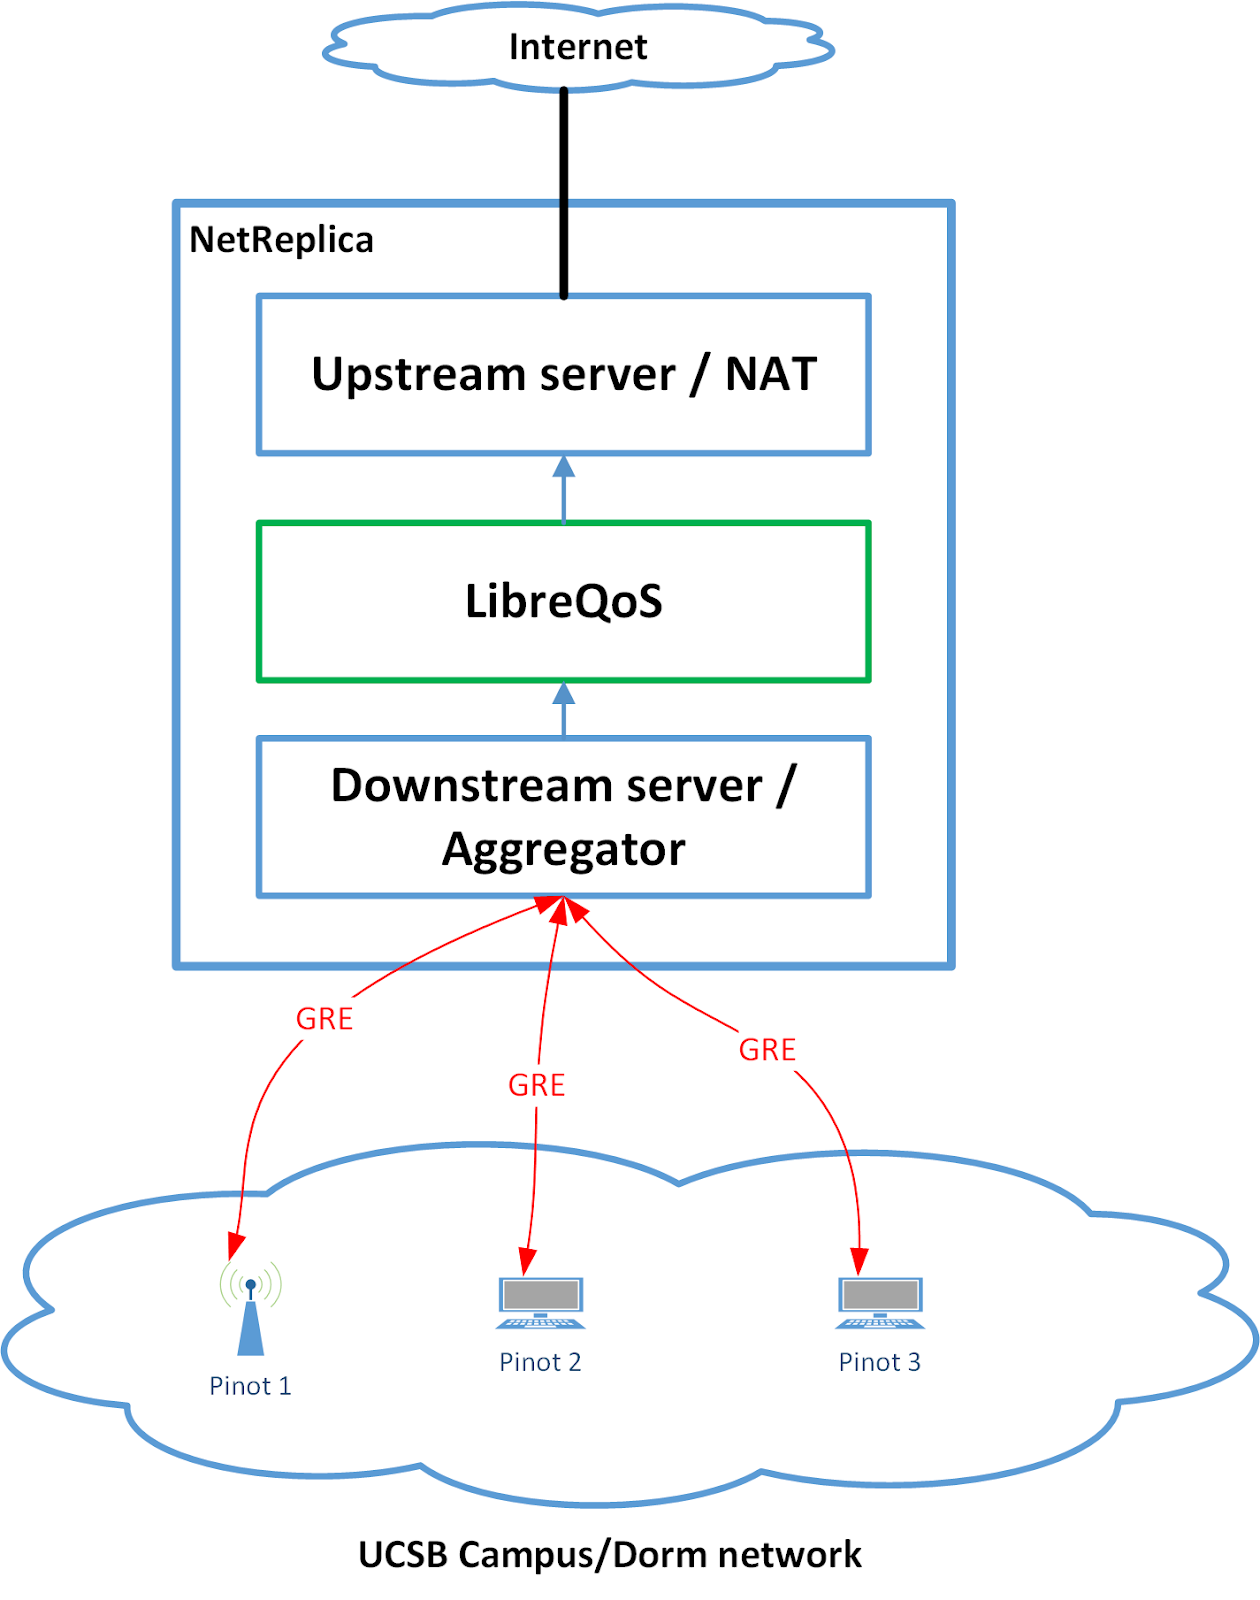
\includegraphics[width=0.4\textwidth]{figures/netReplica.png}
    \caption{netReplica Architecture}
    \label{fig:netReplica}
\end{figure}



Controlling available bandwidth alone does not accurately replicate real network conditions. Each hop from source to destination encounters background traffic from other users sharing network resources. For instance, in a home network, family members using the internet simultaneously can limit bandwidth and increase latency. The same applies to enterprise networks and ISPs, where multiple users access services concurrently, affecting application behavior and packet traces.
Realistic background traffic is crucial for accurate network condition simulation. In applications like video streaming, Adaptive Bitrate (ABR) algorithms may choose lower bitrates to prevent rebuffering under heavy network load. Even if application logic remains unchanged, packet traces are still affected; some packets experience more delay, interarrival times and the number of retransmissions may vary, and other metrics can also be impacted.
For these reasons, a realistic platform controlling network conditions must incorporate authentic background traffic that mimics real-world scenarios.

\subsection{Existing Approaches}
\begin{enumerate}
    \item No Background Traffic: Some studies neglect background traffic, resulting in datasets that fail to capture realistic traces and experiments.
    \item Steady Stream of Flows: Some studies use tools like iperf to create a steady stream of  background traffic with specific throughput. This method fails to represent the bursty nature of real network traffic.
    \item Probabilistic Models: Using Gaussian, Laplacian, or other distributions to generate bursty background traffic is an improvement. However, these models do not reflect real user behavior, as the bursts are not based on actual network traffic distributions.
    \item Trace-based Methods: Some approaches derive traffic distribution from input traces captured from real users using the internet and attempt to mimic it. While better, these methods often rely on simulation environments like MahiMahi, which have their own limitations. These limitations are discussed in subsequent sections.
\end{enumerate}

To create realistic background traffic that accurately mimics real user behavior, we use UCSB network traffic as background traffic. We select a subset of the captured traffic and replay it using the tcpreplay tool in our system while running the controlled application. 
We first captured traffic from the UCSB campus network, including dormitories, at the gateway of UCSB AS for 15 minutes. We collected MAC, IP, and transport layer headers, truncating payloads for privacy and performance while retaining the original packet length. Using PacketSplitter, we separated the captured data based on flows identified by 5-tuples and grouped them by internal IP address. Given that UCSB is one of the early hubs of the internet and has a large block of public IPv4 addresses, most users have unique public addresses, and there is limited network address translation (NAT) in place.
Next, we used CICFlowMeter to extract features from each flow pcap. Our tool, UserActivityAnalyzer (UAA), then analyzed user behavior based on CICFlowMeter output for all flows associated with each user. The extracted metrics included total forward/backward bytes, throughput, number of unique ports used, and distribution of active and idle times, among others.



\subsection{Experiment Design}
We are considering 3 different scenarios to evaluate the performance of this system using netReplica. 
\begin{itemize}
    \item Scenario 1: Wired vs. Wireless nodes 
    \item Scenario 2: Nodes with different distances to the bottleneck 
    \item Scenario 3: Limiting the bandwidth vs. not limiting the bandwidth
    \item Scenario 4: With/without background traffic
    \item scenario 5: Low burst background traffic vs. High burst background traffic
    \item scenario 6: Creating congestion in the access link 
    \item scenario 7: Utilizing different AQM algorithms at the bottleneck link
    \item scenario 8: Separating shaping bottleneck and background traffic bottleneck
\end{itemize}
\input{evaluation}
\section{Measurement Study}
We conduct a study where we characterize the location of the bottleneck link as measured by popular speed test tools. We focus on two such tools, namely Ookla Speed test and M-Lab Network Diagnostic Test (NDT). In addition, we focus on the question whether the bottleneck link is within the last-mile ISP or upstream. We use the Netrics platform for these measurements. 

\textbf{Data Collection}: 
Describe Netrics deployment, including number of tests, time period of the study, number of vantage points. 

Testing setup. Why we are measuring from the client side. What are the implications. 

\subsection{Results}

The data reveals interesting differences between the two tools. The last-mile ISP is the bottleneck for xx\% tests in Ookla, while this number is yy\% in MLab. Further dissecting them by the speed tests, the difference between the two tools increases. 

\section{Related Work}\label{sec:related}

\subsection{Identifcation and Counting of Hosts Behind NAT Using Machine
Learning \cite{shukla2022identification}}
In this, we use ICS data set to train our model which contains traffic flow from 1116 hosts. We identify each host with
the help of source IP address and mark them as a unique
class. Once classes are assigned to each fow, we train our
model with the help of ICS data set. After training our data
model, we have used diferent data sets which contains NATted trafc flow from multiple hosts to test our trained model.
Our trained model then classifes each fow to a class with
the help of all the selected features. Unique classes are then
counted to count number of hosts.

How long the duraiong of ICS dataset? is 400MB enough? It had 460K flows, not natted

The second dataset, MTA: 143 hosts, natted, and non natted
The third dataset, their own, 73 PC hosts 6 hours, natted and non natted, only web, running a script 
The test 

The paper relies heavily on reference 17 for choice of flow analayzer, choice of filtering method 

Much different featurs than us, we are getting mostly the inter-arrival time and flow based stats while the paper gets mostliy thibngs related to window size and ACks. 
ALso, they only not consider src port, but destination port is considered. 

Do they consider UDP packets? Their most important features are tcp

Why not considering all the features and then eliminating shortcuts?
They also had to reduce the number of features and it improved the preformance --> maybe they did not have large enough dataset --> their dataset size is equal to number of flows but ours can be as big is n chose 2 (half of n squared): They use multiclass calssifier 

It redifines some ML stuff to just fill out the paper 

They got 98 percent accuracy when test and train performed on ICS dataset, it is a shortcut though, accuracy dropped to 89 on lab dataset 




IMPORTANT: Tranalayser considers the IAT 

Many of them use NetFlow dataset which is not a good one. 

\subsection{Identifying NAT Devices to Detect Shadow IT: A Machine Learning Approach \cite{nassar2021identifying}}
It's only a binray classification, whether there is a NAT or not.

Instead of identifying NAT behavior based on the features extreacted from traffic traces per flow, it uses ML on aggregated flow features. Also, consider different window sizes for aggregating the flow features. They claim they reached accuracy of 96.9\% on their dataset which we believe it is due to shortcuts and spurious correlations. They claim that using the extractd featres from the flow resulted in high false positive rate; but we calim that although it might be true, it is not true when using correct set of featuers and the method that we have.  For example, if the algorithm is using TTL value as a feature to detect NAT, some NAT devices are deployed in a way that could not decrement the TTL (they mention it for pervious work). TTL can be useful in detecting NAT along the other features but solely relying on it is not a good idea. 
While the paper claims that Aggregating features increase the classification accuracy because it increases the chance of having more than one active user, we showed that this method resulted in a very samll dataset and it is not a good idea. 


The dataset issue; The dataset, “NAT Network Traffic Dataset”, is composed of 294 capture files from 294 tests done. It was collected over two weeks in June 2020, with three sessions per day. Each session, morning, midday, and evening, consists of 7 different tests done by varying the devices connected to the NAT router and the application opened by devices behind 
NAT. Because of these issues and not having a realistic dataset to validate their model, we believe that their model is not generalizable and the reported accuracy is not reliable.

This dataset is not big enough, is not diverse enough, and it is based on synthetic data. As a result, one obviouse issue is that the model uses average packets recieved and average bytes recieved as the main features to detect NAT. This is a shortcut and it is not a good idea.

\subsection{A Generalizable Machine Learning Model for NAT
Detection \cite{nassar2023generalizable}}
Same auther as \cite{nassar2021identifying}

Based on their previous work, it is just detecting the existences of NAT, not complete set of features, users transfer learning, not a good dataset. Their passive setup has the same issue as the prvious dataset, it is not diverse enough, it is small and based on synthetic data.

Outdated method, that used scapy instead of CICFlowMeter, it is slower and does not caputre all the features that we need. It uses limited set of features obtained from the packets and not the flows. They only consider 1 minutes of data, which is not enough. Because of these issues and not having a realistic dataset to validate their model, we believe that their model is not generalizable and the reported accuracy is not reliable.



\subsection{Exploring nat detection and host identification using machine learning \cite{khatouni2019exploring}}

check this paper: Integrating machine learning
with off-the-shelf traffic flow features for http/https traffic classification,

Also based on this paper, tranalyzer had the best preformance. They used several tools, maybe breifly mention them. Spent most of the paper defining the F1 score, recall and precision which is not needed. They are also reporting 98 percent accuracy which is not reliable. No details about the dataset, 

Poor dataset (figure 1 for create dataset). Not big enough (maybe), not diverse enough, based on synthetic data. They just mention 300GB of data with NAT and without NAT. 
There are 16 hosts equipped with either Kali Linux Rolling4 or Microsoft Windows 7 Professional operating systems. Furthermore, there are two network configurations for the testbed set up: (i) Network with NAT; and (ii) Network without NAT. In the first configuration, each host is connected to a switch then these connections pass through a NAT and Dynamic Host Configuration Protocol (DHCP) server to access the public Internet. Used iMacros, which is synthetic data. 

use limited number of features for training, only 8 of them, only works with tcp cause many of the main features are tcp related. Besides, it is not for detecting number of users behind the NAT, it just sasy whether there is a NAT or not.

Not sure how they are using the flow level information, are they aggregating them or they assign every flow is behind a NAT or not? 



\subsection{How Polynomial Regression Improves DeNATing \cite{adler2023polynomial}}
The refrences one to 9: check them all

The main ID of using IPID sucks: One is because of concurrent connections, it weould not get increamented but it would increase a lot in time, the other thing is DNS resovler in the network behind NAT and also DNS caching 

It is TCP/IP based, what about UDP 

Identifying packets belong to the same flow using TCP timestamp: Isn't it already solved by 4 tuples using pcapsplitter or cicflow?


Assumption about IP IP assignmet by increameing it for each packet either per flow or globally

They use TTL that can be a shortcut, but what about different devices use differnt Initial TTL: This can be a good info 

Check the TCP window Scale size 

OS fingerprinting using TCP/IP header fileds 

Communication with speficif domains for OS fingerprinting (ref 15)

check netflow records 

Check Timestamp filed and the two studies based on timestamp

In old versions of Windows OS, the IP-ID field was
implemented as a simple counter. Newer versions use separate
counters per destination address. IOS assigns a random number
to IP-ID, and some versions of Linux always set it to zero.

The IP-ID method requires long time of catpuring data cause for creating sequence I guess they need more than several DNS requests. Also, how precies is that?


ntegrating machine learn- ing with off-the-shelf traffic flow features for http/https traffic classifica- tion,

just http / https 
\section{Discussion}
Discuss the limitations and future work here.

\textbf{Explaining errors}

\textbf{Generalizability of methodology to different tests and device platforms}

\textbf{Generalizability of the measurement study}
\section{Conclusion}\label{sec:conclusion}


\begin{acks}
To Robert, for the bagels and explaining CMYK and color spaces.
\end{acks}

%%
%% The next two lines define the bibliography style to be used, and
%% the bibliography file.
\bibliographystyle{ACM-Reference-Format}
\bibliography{paper}

\end{document}
\endinput
%%
%% End of file `sample-sigconf.tex'.
